\chapter{Conclusione \workinprogress}

\begin{comment}
Conclusioni

Al momento di scrivere le conclusioni spesso si rimette mano anche all'introduzione poiché sono due sezioni tra loro collegate. Non occorre ripetere quindi le conclusioni già inserite eventualmente nei vari capitoli, ma piuttosto inserire una breve analisi del lavoro svolto, delle problematiche affrontate e delle metodologie per risolverle e indicare possibili futuri sviluppi.

scaletta
    1. sta tesi è una guida implementativa
    2. sta architettura è stata implementata su apparati reali
    3. per la tesi l'architettura è stata simulata
        1. quindi ci stanno delle differenze, es ho usato openwrt stock
    4. evoluzione futura multi-istanza usando una pki perogni processo vpn


\end{comment}

L'architettura proposta in questo elaborato è stata effettivamente implementata su apparati reali durante il tirocinio in collaborazione con l'azienda \textit{Esse-ti}. Ciò ha permesso, a me e hai miei colleghi, di lavorare a stretto contatto con un'azienda del territorio, tenendo conto dei loro requisiti e limiti di budget.


Personalmente questo progetto mi ha permesso di espandere la mia conoscenza sul mondo del networking e di Linux. Affrontando le sfide causate dalla configurazione di un server remoto e un dispositivo di tipo embedded.


In fase di revisione con il responsabile aziendale è emersa una limitazione dell'architettura implementata, può infatti sostenere un solo cliente e il relativo router 4G. Per sostenere più di un cliente sarebbe necessario avere più di una VPS e ripetere la procedura di configurazione in ognuna. 

Se si vuole consentire l'uso di una sola VPS per più clienti è necessario implementare una multiistanza VPN, in cui ogni VPN è dedicata ad un solo cliente e relativo router. Possiamo vedere un prototipo della topologia reale e virtuale in fig.~\ref{fig:diag2-multiistanza_virtual} e fig.~\ref{fig:diag2-multiistanza_real}. In questo caso si deve porre particolare attenzione alla sicurezza, in quanto si deve garantire l'isolamento assoluto tra clienti differenti. La chiave per l'implementazione della multiistanza è di avere una \it{Certificate Autority} separata per ogni VPN, ciò comporta che i clienti possano autenticarsi solo alla VPN che gli è stata assegnata.


\todo[manca frase conclusiva]

\begin{figure}
    \centering
    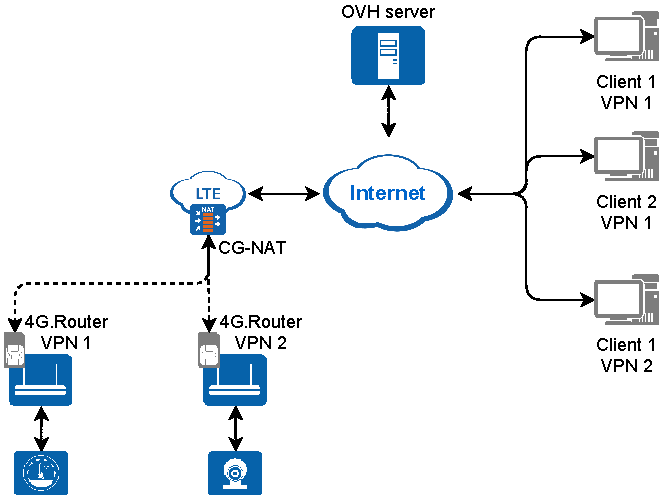
\includegraphics[width=0.8\linewidth]{immagini/diag2-multiistanza_real}
    \caption{Prototipo di topologia reale della multiistanza VPN}
    \label{fig:diag2-multiistanza_real}
\end{figure}

\begin{figure}
    \centering
    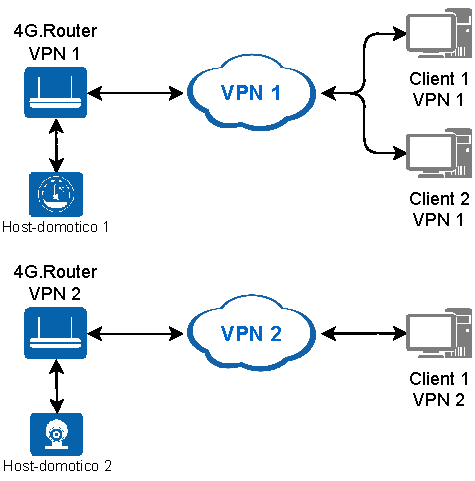
\includegraphics[width=0.6\linewidth]{immagini/diag2-multiistanza_virtual}
    \caption{Prototipo di topologia virtuale della multiistanza VPN}
    \label{fig:diag2-multiistanza_virtual}
\end{figure}





